\section{Protótipo de Baixa Fidelidade}

A Figura~\ref{fig:prototipo} apresenta o protótipo de baixa fidelidade da interface web do sistema. Ele serve para definir a organização geral da página e o fluxo de interação com o usuário, sem detalhes visuais finais como cores, tipografia e identidade visual.

A página inicial dá boas-vindas ao usuário e apresenta três botões, um para cada modo de operação: Ligado, Automático e Desligado. Ao selecionar um modo, a tela passa a exibir os valores de temperatura e umidade, identificados por ícones, junto de uma mensagem de estado:

\begin{itemize}
    \item \textbf{Modo Ligado:} exibe as leituras de temperatura e umidade em tempo real;
    \item \textbf{Modo Automático:} exibe as leituras e a mensagem ``Atualizando...'', indicando que os dados são renovados continuamente, e que o sistema opera de forma autônoma;
    \item \textbf{Modo Desligado:} não exibe leituras e mostra a mensagem ``Sensores Desligados!'' em destaque.
\end{itemize}

\begin{figure}[!htb]
    \centering
    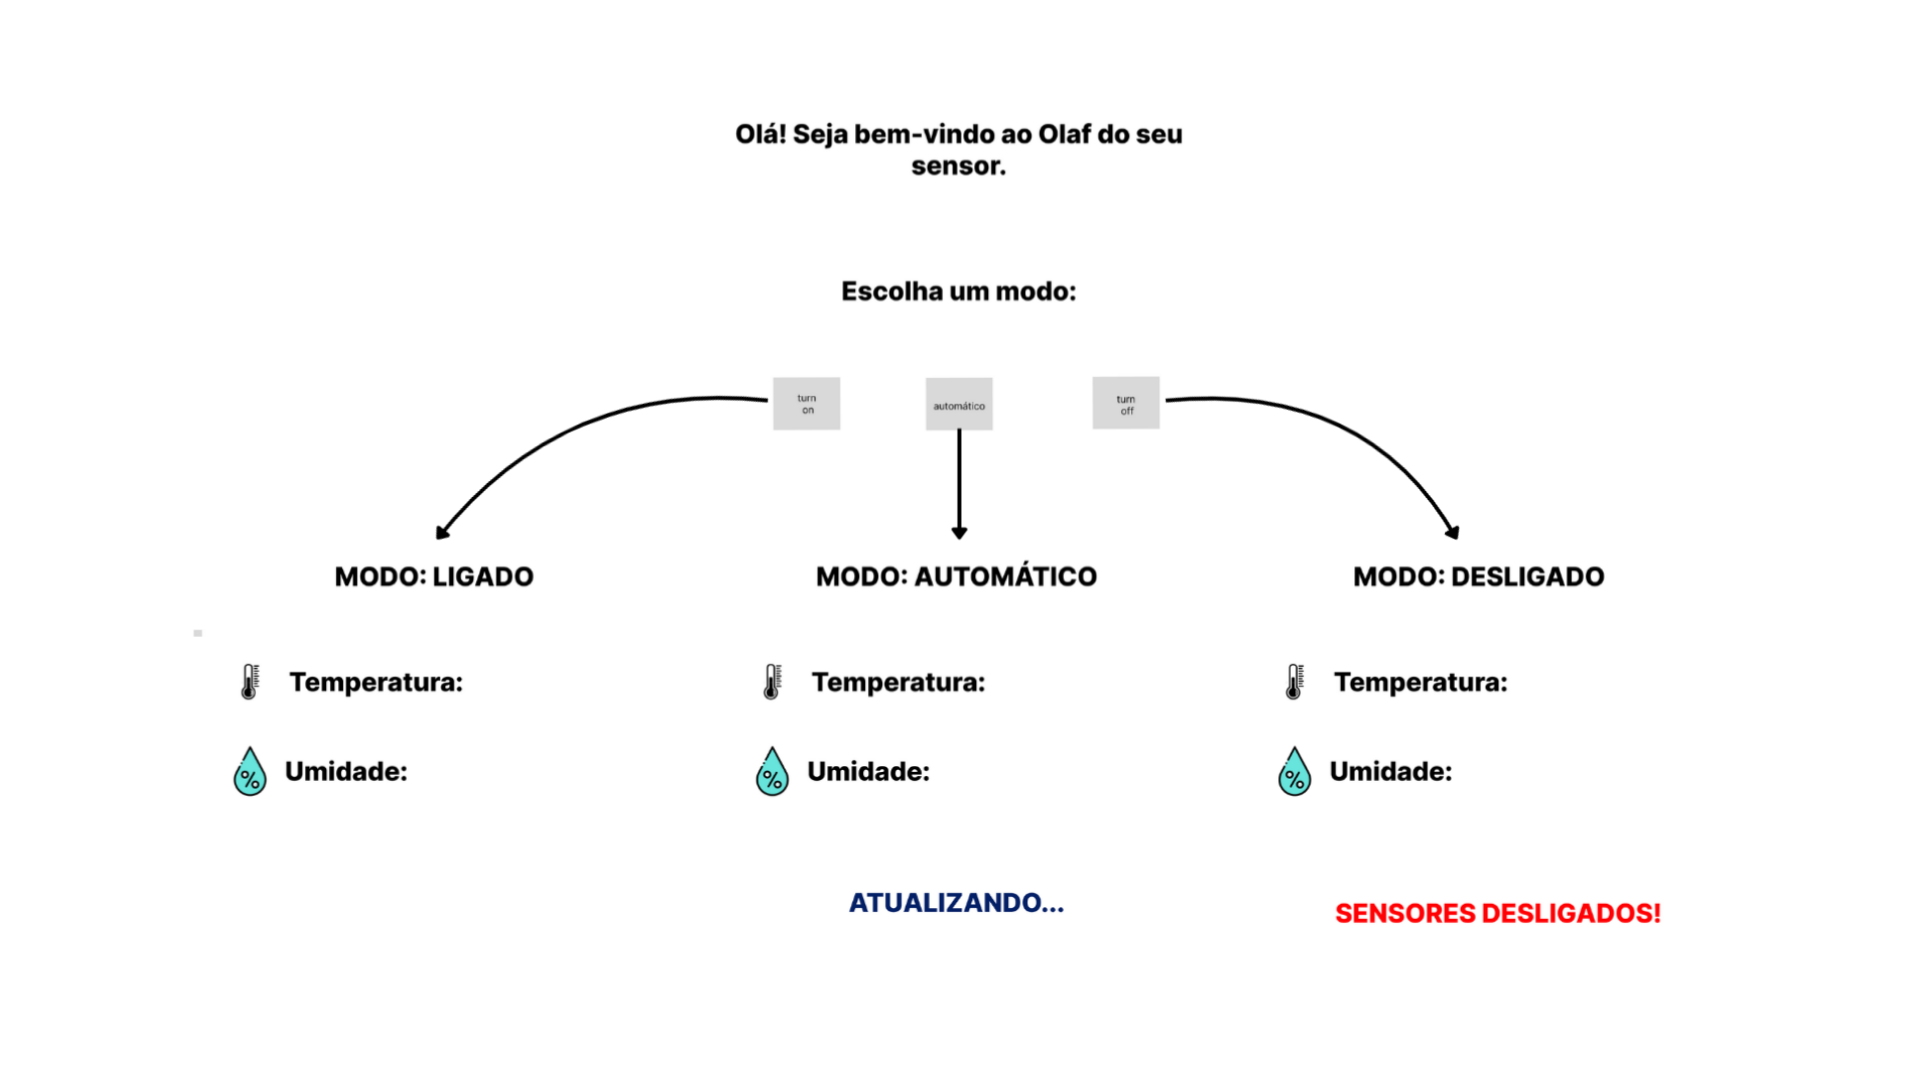
\includegraphics[width=\textwidth]{imag/prototipo.png}
    \caption{Protótipo de baixa fidelidade da interface web.}
    \label{fig:prototipo}
\end{figure}